\documentclass{article}
\usepackage[a4paper,bindingoffset=0.2in,%
            left=1.1in,right=1.1in,top=1.1in,bottom=1.1in,%
            footskip=.25in]{geometry}
\usepackage{graphicx}
\usepackage{indentfirst}
\usepackage{caption}
\usepackage{subcaption}
\begin{document}

  \begin{titlepage}
  	\centering
  	{\huge\bfseries STA 135 Final Project\par}
  	\vspace{2cm}
  	{\Large\itshape Siqi Bian (Susie)\par}
    \vspace{0.5cm}
  	{\Large\itshape Huang Fang\par}
    \vspace{0.5cm}
  	{\Large\itshape Wenyu Li\par}
  	\vspace{0.5cm}
  	{\Large\itshape Zhen Zhang\par}
  	\vfill

  	\vfill
  	% Bottom of the page
  	{\large \today\par}
  \end{titlepage}

  \newpage

  \section{Introduction}

    In this project, we are given the data of diagnosis of depression in primary care, from which we learn different components and diagnosis results. The components consist of physical component, mental component, beck depression score, patient gender, age, and number of years of formal schooling. We need to study for each of these components, how they play a role in determining the result of diagnosis, from different perspectives, such as regression, principle component analysis and discriminant analysis.
  \section{Material and Methods}
    Here we draw histograms, qqplots and boxplots (See Appendix I). From the histograms and qq plots of each variable, we find that the most variables are skewed, but not severe. So it is not necessary to apply any transformation to the variables. From the boxplots, we can find that ``mcs" and ``beck" seem to have different distribution under different levels of ``dav", patients with less ``mcs" and more ``beck" tend to diagnosed. On the contrary, ``pcs" and ``age" seem to have no impact on ``dav".

    First we analyze whether these components are significant in the result of diagnosis, and whether they differ from each other when categorized into different education levels. Here we calculate the Hotelling's T from the deviation between each categories of each variable and their variance, and then compare the results with the corresponding F-value. When there are multiple comparisons we need to do, we use MANOVA to do multivariate comparison.

    After these qualitative procedures, we use multivariate regression model, principle component analysis and linear discriminant analysis to analyze the data quantitatively. For multivariate regression model, we select MCS and BECK as the response variable and PCS, AGE and GEND as the independent variable. For principle component analysis, we get the most important combined variable, and how each component determine it. For linear discriminant analysis, we use it to categorize the diagnosis status by PCS, MCS, BECK and AGE.
  \section{Results}
    \subsection{Compare Mean Vectors}
      We assume $p\times p$ population covariance matrices are equal and of full rank. Then we apply $T^2$ statistics to test the equality of vector means from two multivariate populations.

      $$T^2 = [\bar{X_1} - \bar{X_2}]^T [(\frac{1}{n_1} + \frac{1}{n_2})S_{pooled}]^{-1} [\bar{X_1} - \bar{X_2}] = 55.31641$$
      $$F^* = \frac{(n_1 + n_2 - 2)p}{n_1 + n_2 - p - 1}F_{p, n_1 + n_2 - p - 1}(0.05) = 9.487729$$
      $H_0: \mu_1 - \mu2 = 0 ~ vs. ~ H_a: \mu_1 - \mu2 \neq 0$

      By comparing of the mean vectors of continuous measurements (PCS, MCS, BECK and AGE ) between those diagnosed as depressed and those that have not been diagnosed, we have the F statistics larger than the threshold, meaning  we should reject the null hypothesis, conclude that PCS, MCS, BECK and AGE have an influence on the diagnosis of depression.

      Then we use the MANOVA method to compare the mean vectors of different education groups:

      \begin{center}
      \begin{tabular}{c c c c c c c}
        \hline
         & Df & Wilks & approx F&num Df&den Df  &  P-value\\
        \hline
        $edu_{encode}$ & 1 & 0.94083 & 6.2101   &   4   & 395 & 7.449e-05\\
        \hline
      \end{tabular}
      \end{center}

      The Wilks test told us that the P-value = 7.449e-05, which means that the four measurements above differ significantly in different education groups.

    \subsection{Multivariate Regression}
      First, we apply multivariate regression of MCS on PCS, AGE and PGEND.

      The summary table suggests that only "pgend" is significant among all the variables, so we can drop "pcs" and "age" from our model.

      \begin{center}
      \begin{tabular}{c c c c c}
        \hline
          &Estimate&Std. Error    & t value & p-value\\
        \hline
          (Intercept)& 40.25626 &3.1975& 12.5899& 8.36e-31\\
          pcs & 0.05524& 0.0561 & 0.9840& 3.26e-01\\
          age & 0.00295& 0.0421 & 0.0699& 9.44e-01\\
          pgend1& 4.95336& 1.3119 & 3.7758& 1.84e-04\\
        \hline
      \end{tabular}
      \end{center}

      Our regression function for MCS is: $MCS = 40.26 + 4.96\times GEND$

      Then we fit BECK on PCS, AGE and PGEND.

      \begin{center}
      \begin{tabular}{c c c c c}
        \hline
          &Estimate&Std. Error & t value & p-value\\
        \hline
          (Intercept)& 11.5588& 1.3843 & 8.35 & 1.16e-15 \\
          pcs & -0.1200& 0.0243 & -4.94 & 1.18e-06\\
          age & -0.0148   &  0.0182&  -0.81 & 4.19e-01\\
          pgend1& -1.5221  &   0.5679 & -2.68  & 7.67e-03\\
        \hline
      \end{tabular}
      \end{center}

      For "beck", both "pcs" and "pgend" are significant, and "age" can be dropped.

      The regression function for BECK is: $BECK = 11.56 - 0.12\times PCS - 1.52\times GEND$

    \subsection{Principal Components Analysis}

      Then we would like to do a principal component analysis on variables PCS, MCS and BECK. After comparing the scales of these three variables, we can find they don't vary widely. Under this situation, we don't need to consider scaling them prior to the application of principal components analysis. We calculated the coefficients of the linear combinations of the continuous variables. From the principal components analysis plot, we can see that the first two PCs explain most of the variability in the data. Here is our rotation table:

      \begin{center}
      \begin{tabular}{c c c c}
        \hline
        & PC1 & PC2 & PC3\\
        \hline
        1 & -0.289 & -0.95156 & -0.105\\
        2 & -0.902 & 0.30736& -0.302\\
        3 & 0.320 & 0.00779 & -0.948\\
        \hline
      \end{tabular}
      \end{center}

      The Figure below is useful to decide how many PCs to retain for further analysis. In this simple case with only 3 PCs this is not a hard task and we can see that the first two PCs explain most of the variability in the data. Also we give a visualization of our vectors.

      \begin{figure}[htb!]
        \centering
        \begin{subfigure}{.5\textwidth}
          \centering
          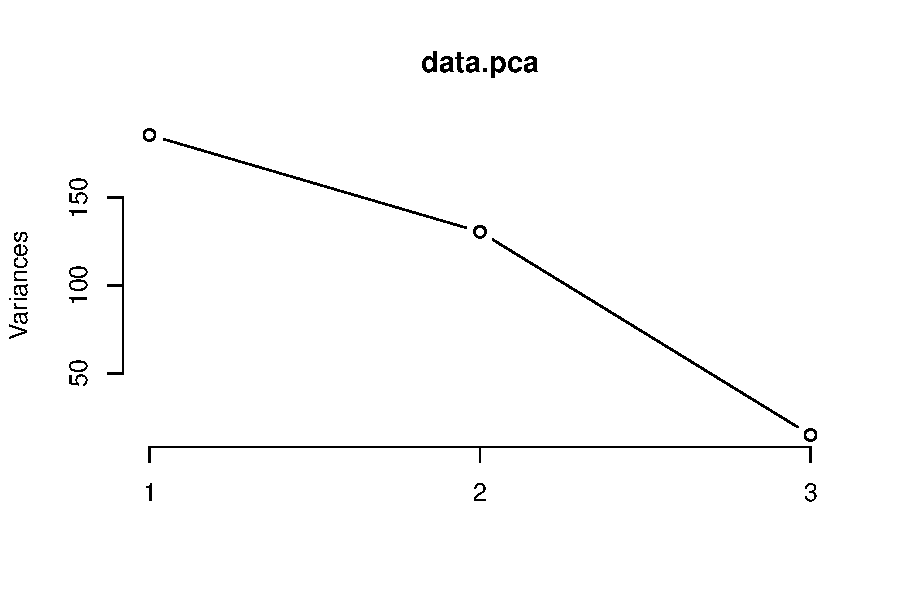
\includegraphics[width=1.2\linewidth]{image1.pdf}
          \caption{Variance explained}
          \label{fig:sub1}
        \end{subfigure}%
        \begin{subfigure}{.5\textwidth}
          \centering
          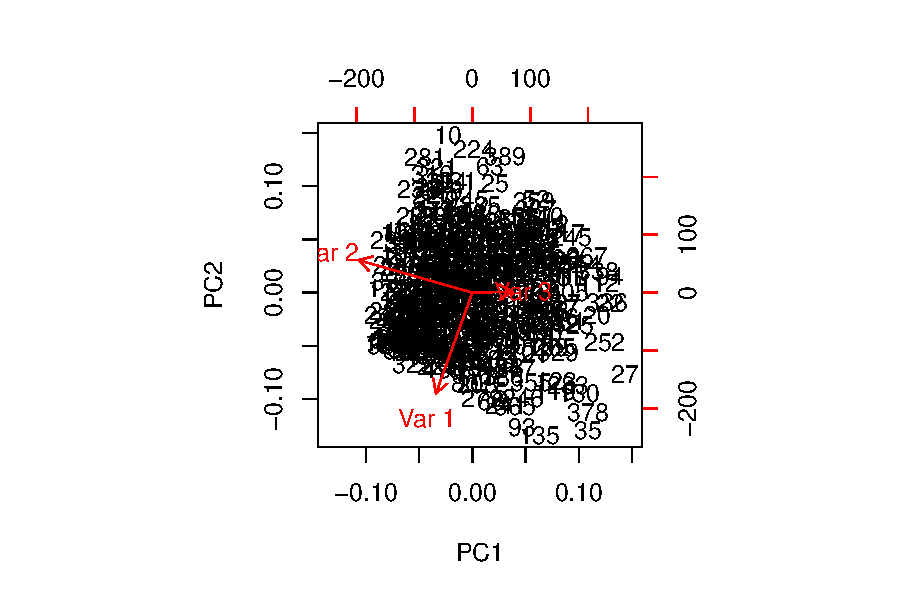
\includegraphics[width=1.2\linewidth]{image2.pdf}
          \caption{Vector visualization}
          \label{fig:sub2}
        \end{subfigure}
        \caption{PCA Figures}
        \label{fig:test}
      \end{figure}

      The summary tells the importance of the principal components. The first row describe again the standard deviation associated with each principal component. The second row shows the proportion of the variance in the data explained by each component. The third row describe the cumulative proportion of explained variance. We can see there that the first two PCs accounts for more than 95\% of the variance of the data.

      \begin{center}
        \begin{tabular}{c c c c}
          \hline
          &PC1 &   PC2   &PC3\\
          \hline
          Standard deviation &    13.625& 11.426& 3.862\\
          Proportion of Variance & 0.561&  0.394& 0.045\\
          Cumulative Proportion&   0.561&  0.955& 1.000\\
          \hline
        \end{tabular}
      \end{center}

    \subsection{Fisher's discriminate analysis}
      Assume the population covariance matrices are equal and of full rank. First, we select DAV, PCS, MCS, BECK and AGE from the whole dataset for building Fisher's Discriminant test. Then we calculate $\bar x_1$ and $\bar x_2$:

      \begin{center}
        \begin{tabular}{c c c c c}
          \hline
          &pcs  & mcs&  beck&   age\\
          \hline
          $\bar x_1$ & 41.54 &46.41 & 4.66 &41.89\\
          $\bar x_2$ & 38.77 &35.00 & 9.36 &43.66\\
          \hline
        \end{tabular}
      \end{center}

      Then after the computation of the sample between groups sums of cross products B and the sample within groups sums of cross products $W$, we choose $s \leq min(g-1,p) = 1$ nonzero eigenvalue of $W^T B$ and its corresponding eigenvector $\hat \alpha_1$. Finally, normalize $\hat \alpha_1$ to make $\hat \alpha_1^T S_{pooled} \hat \alpha_1$ = 1. Here is the normalized $\hat \alpha_1$.

      \begin{center}
        \begin{tabular}{c c c c c}
          \hline
          a & -0.00729 &-0.05422 & 0.07699 & 0.00800\\
          \hline
        \end{tabular}
      \end{center}

      Therefore, the corresponding discriminant function is

      $$y = ax = -0.00729X_1 -0.05422X_2 + 0.07699X_3 + 0.00800X_4$$

      Next we can compute the misclassification rate, which is 0.275

      Finally we made the four-dimension into an one dimensional plot. Here we can see almost red points are located left and blue points are distributed scatteredly. Thus if the LD value is very small, then the variable is more likely to be not diagnosed.

      \begin{figure}[htb!]
        \centering
        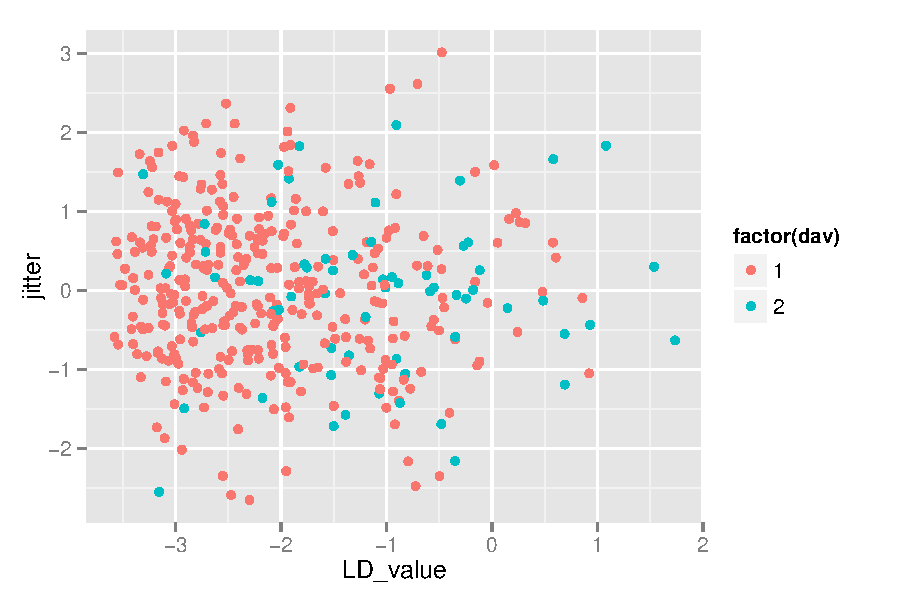
\includegraphics[width=0.8\linewidth]{image3.pdf}
        \caption{Fisher Discriminant Analysis}
      \end{figure}
  \section{Conclusion and discussion}
    According to the analysis we have conducted, there are some conclusions obtained from the results. Firstly, the physical and mental component of the patient with SF-36 heath status, the beck depression score and their age have significant influence on the diagnosis depression. Then, we found those above four measurements differ significantly in different education groups. Next, by conducting multivariate regression analysis, we obtained the significant linear regression relationship respectively on the mental component with the gender and on the beck depression score with the physical component and the gender. After that, we did the principal component analysis on the physical and mental component and the beck depression score, from which we concluded that the first two components explained 95.5\% variability of the data. At last, we performed the Fisher's discriminate analysis on the physical and mental component, the beck depression score and the age for classifying if the patient is diagnosed or not. By obtaining the discriminant function, we achieved the misclassification rate 27.5\% on the classification.
\end{document}
